%\documentclass{beamer}
\makeatletter\let\ifGm@compatii\relax\makeatother
\documentclass[ignorenonframetext]{beamer}
\mode<presentation>
% Copyright 2003 by Till Tantau <tantau@cs.tu-berlin.de>.

\usetheme{Aston}
%\usetheme{Berkeley}

\usepackage{subfigure}
\usepackage[english]{babel}
\usepackage[latin1]{inputenc}
\usepackage{beamerthemesplit}
\usepackage{booktabs}
\usepackage{amsmath} % We will always use the amstex package!
\usepackage{xspace} % Xspace is very useful to, thanks Guillaume!
\usepackage{chicagoMod} % for bibliography

\usepackage{data_assimilation}
%\usepackage{gp}

\newcommand{\mbf}	 {\boldsymbol}
\newcommand{\enclose}[1] {{\it \lq #1\rq }\xspace}
\newcommand{\degr}[1]	{\ensuremath{#1^{\circ}}\xspace}
\newcommand{\trans}[1]	{\ensuremath{#1^{\text \tiny T}}\xspace}
%\newcommand{\pxgy}[2]	{\ensuremath{\text{p}(#1\: | \: #2)}\xspace} % conditional probability of x given y
\newcommand{\pxay}[2]	{\ensuremath{\text{p}(#1,#2)}\xspace} % joint probability of x and y
\newcommand{\px}[1]	{\ensuremath{\text{p}(#1)}\xspace} % probability of x
\newcommand{\approxpx}[1]	{\ensuremath{\text{q}(#1)}\xspace} % probability of x
\newcommand{\approxpxgy}[2]	{\ensuremath{\text{q}(#1\: | \: #2)}\xspace} % probability of x
\newcommand{\pbayes}[2]	{\ensuremath{\frac{\pxgy{#2}{#1}\px{#1}}{\px{#2}}}\xspace} % posterior probability of x given y
\newcommand{\gaussoned}[3]  {\ensuremath{\frac{1}{\sqrt{2\pi #2}} \exp\left(-\frac{(#3-#1)^2}{2 #2}\right)}\xspace}  
\newcommand{\propdist}	{\ensuremath{\hat{\text{q}}()}\xspace} % probability of x


\newcommand{\prd}	{probability distribution\xspace}
\newcommand{\prds}	{probability distributions\xspace}
%\newcommand{\pdf}	{probability distribution function\xspace}
\newcommand{\pdfs}	{probability distribution functions\xspace}


\newcommand{\mean}{\ensuremath{\mu}\xspace}
\newcommand{\bd}{\ensuremath{\mbf{D}}\xspace}
\newcommand{\expect}[1]	{\ensuremath{E\left[#1\right]}\xspace} % expectation
\newcommand{\bw}	{\ensuremath{\mbf{w}}\xspace} 
\newcommand{\bt}	{\ensuremath{\mbf{t}}\xspace} 
\newcommand{\bx}	{\ensuremath{\mbf{x}}\xspace} 
\newcommand{\by}	{\ensuremath{\mbf{y}}\xspace} 

\renewcommand{\emph}[1]		{{\color[rgb]{0.5804,0.1569,0.5451}#1}}
\newcommand{\defn}[1]		{{\color[rgb]{0.5804,0.1569,0.5451}#1}}
\newcommand{\imp}[1]		{{\color[rgb]{0.0000,0.2353,0.4745}#1}}
\newcommand{\pers}[1]		{{\color[rgb]{0.0,0.3,0.3}#1}}

\newcommand{\samplemean}        {\ensuremath{\hat{\mu}}\xspace}	% finite sample mean


\newcommand{\outlineMark}[1]		{{\Huge \color[rgb]{1.0,0.3,0.3}#1}}

\newcommand{\dint}		{\mathrm{d}} % d integral 
\newcommand{\tr}		{\mathrm{tr}} % trace
\newcommand{\diag}		{\mathrm{diag}} % trace
\newcommand{\FIM}       {\ensuremath{\mathcal{F}}\xspace}
\newcommand{\qi}{ {\tau } \xspace} % quantile index

\newcommand{\Nkn}{ { N_{k,-i} } }
\DeclareMathOperator*{\argmin}{arg\,min}

\newcommand{\z}       {\ensuremath{\mathbf{z}}\xspace}
\newcommand{\conc}       {\ensuremath{{\alpha}}\xspace}
\newcommand{\thp}        {\ensuremath{\mathbf{\theta}_0}\xspace}

%%% END : Put your own macro's here
%%%%%%%%%%%%%%%%%%%%%%%%%%%%%%%%%%%%%%%%%%%%%%%%%%%%%%%%%%%%%%%%%%%%%%%%%%%%%%%
% Remi's stuff ...
\definecolor{turquoise}{RGB}{25,106,175}
\definecolor{orange}{RGB}{240,100,50}
\definecolor{green}{RGB}{0,128,0}
\definecolor{urlgray}{RGB}{100,100,100}


\renewcommand{\emph}[1]{{\color{turquoise} #1}}
\newcommand{\textorange}[1]{{\color{orange} #1}}
%\newcommand{\pictureurl}[1]{\tiny{\color{urlgray} #1}}
\newcommand{\pictureurl}[1]{\ \footnote[frame]{\tiny{\color{urlgray} #1}}}
\newcommand{\rarrow}{$\rightarrow$\ }
\newcommand{\mc}[1]{\ensuremath{\mathbf{#1}}\xspace}

%\setbeamercolor{block title}{bg=blue}
%\setbeamercolor{background canvas}{bg=yellow} % see http://en.wikibooks.org/wiki/LaTeX/Presentations
%\setbeamercolor{block body alerted}{bg=yellow}
%\setbeamercolor{block body}{bg=red}
\setbeamercolor{block head}{bg=blue,fg=white}
%\setbeamercolor{block body example}{bg=green}
%\setbeamercolor{block title alerted}{bg=black}
%\setbeamercolor{block title}{bg=brown}


\newcommand{\xinput}        {\ensuremath{\mc{x}}\xspace}
\newcommand{\Xinput}        {\ensuremath{\mc{X}}\xspace}
\newcommand{\youtput}        {\ensuremath{\mc{y}}\xspace} 
\newcommand{\proboutput}        {\ensuremath{\mc{\beta}}\xspace} 
\newcommand{\simfn} {\ensuremath{\mc{f}}\xspace}


\newcommand{\der}		{\ensuremath{\partial}\xspace} % partial derivative


\newcommand{\me}        {\ensuremath{\mc{\mu}}\xspace}
\newcommand{\cov}       {\ensuremath{\Sigma}\xspace}
\newcommand{\pa}        {\ensuremath{\mc{\theta}}\xspace}
\newcommand{\X}        	{\ensuremath{\mc{X}}\xspace}

\newcommand{\logvar}{\mc{z}} % log varinace
\renewcommand{\obs}{\mc{t}}	% raw noisy observation
\newcommand{\BasisFun} {\ensuremath{\mc{h}}\xspace}		% fixed basis array
\newcommand{\BasisB} {\ensuremath{\mc{\beta}}\xspace}	% linear params


% Private macros
\usepackage{xspace}

\newcommand{\x}        	{\ensuremath{\mc{x}}\xspace}
\newcommand{\abc} {{\it ABC}\xspace}
\newcommand{\design}        	{\ensuremath{\mc{\xi}}\xspace}

\newcommand{\truemean}        {\ensuremath{{\mu}}\xspace}	% finite sample mean

% Used in ch3 for coupled model
\newcommand{\gpone} {\ensuremath{\mc{G_H}}\xspace}
\newcommand{\gptwo} {\ensuremath{\mc{G_\sigma}}\xspace}
\newcommand{\gpthree} {\ensuremath{\mc{G_{\mu}}}\xspace}
\newcommand{\meanoutput}        {\ensuremath{\bar{y}}\xspace}
\newcommand{\varoutput}        {\ensuremath{\mc{S}^2}\xspace} 
\newcommand{\target}        {\ensuremath{\mc{t}}\xspace}
\newcommand{\yuhba} {\ensuremath{\mc{Y}} \xspace}

\newcommand{\Data} {\ensuremath{\mathcal{D}} \xspace}
\renewcommand{\v}[1] {\mathbf{#1}} % vectors in math mode
\newcommand{\ti} { \mathcal{\tau} }



\newcommand{\myhbox}[1]{ \fbox{\bf {#1} }} 

\graphicspath{{figs/}} 

\newcommand{\arrow}[1][\ ]{\emph{$\boldsymbol{\Rightarrow}$}#1}

%\setbeamercovered{transparent}
\setbeamercovered{invisible}
\setbeamercovered{dynamic}

\newcommand{\cut}[1]{} % remove material from compilation - handy this!

% PDF metadata settings
\hypersetup{%
	pdftitle={MUCM},%
	pdfauthor={Alexis Boukouvalas},%
	pdfsubject={},%
	pdfstartview={FitH},%
	pdfkeywords={}%
}


\title[Branching GPs]{Identification of branching using pseudotime estimation}
\author[A.~Boukouvalas]{\textcolor{darkblue}{Alexis Boukouvalas}\\ \textcolor{blue}{\tt \tiny alexis.boukouvalas@manchester.ac.uk}}
\institute{
  
\includegraphics[height=2cm]{ManchesterUniversityLogo} \hspace{2cm} 
 \\
  \textcolor{blue}{\tt \tiny http://personalpages.manchester.ac.uk/staff/alexis.boukouvalas/}
}
\date{
  \textcolor{darkblue}{August 31, 2016} \\
  Joint work with James Hensman, Magnus Rattray
}


% nice rounded corners
\setbeamertemplate{blocks}[rounded][shadow=true] 

% Make captions red without figure and colon
\setbeamertemplate{caption}{\small \insertcaption}
\setbeamercolor{caption}{fg=blue,bg=white} 

% nice rounded corners
\setbeamertemplate{blocks}[rounded][shadow=true] 

\usepackage{xmpmulti}

% new
\usepackage{pgfplots}
\usepackage[subpreambles=true]{standalone}
\usepackage{tikz}


\begin{document}

% Make the title page.
\frame{\titlepage}


\begin{frame}{Hello world}
%% This file was created by matplotlib2tikz v0.6.0.
\begin{tikzpicture}

\definecolor{color2}{rgb}{1,1.22464679914735e-16,6.12323399573677e-17}
\definecolor{color1}{rgb}{0.503921568627451,0.999981027348727,0.704925546906147}
\definecolor{color0}{rgb}{0.5,0,1}

\begin{axis}[
xmin=-0.2, xmax=1.2,
ymin=-0.0537118855386883, ymax=0.366748907482901,
tick align=outside,
xmajorgrids,
x grid style={white},
ymajorgrids,
axis line style={white},
axis background/.style={fill=white!89.803921568627459!black}
]
\addplot [only marks, draw=color0, fill=color0, colormap={mymap}{[1pt]
  rgb(0pt)=(0,0,0.5);
  rgb(22pt)=(0,0,1);
  rgb(25pt)=(0,0,1);
  rgb(68pt)=(0,0.86,1);
  rgb(70pt)=(0,0.9,0.967741935483871);
  rgb(75pt)=(0.0806451612903226,1,0.887096774193548);
  rgb(128pt)=(0.935483870967742,1,0.0322580645161291);
  rgb(130pt)=(0.967741935483871,0.962962962962963,0);
  rgb(132pt)=(1,0.925925925925926,0);
  rgb(178pt)=(1,0.0740740740740741,0);
  rgb(182pt)=(0.909090909090909,0,0);
  rgb(200pt)=(0.5,0,0)
}]
table {%
x                      y
+3.168065186308531e-03 -1.367480970669057e-02
+6.496218700371184e-03 -1.928193382995866e-03
+7.865377122435501e-03 -1.000950393481593e-03
+9.173192134749991e-03 +4.776919607931678e-04
+1.037500703424895e-02 -1.558787056517283e-02
+1.129538616179000e-02 -1.032503994001920e-02
+1.207715386105559e-02 -1.548341779303444e-02
+1.321547144097784e-02 -2.721184852158029e-02
+1.448734802616245e-02 -2.715624140720754e-02
+1.554169851295343e-02 -2.544036116335210e-02
+1.657472430316785e-02 -1.614618506098601e-02
+2.069572612994217e-02 -1.882974209198878e-02
+2.867055155398853e-02 -2.085734505144796e-02
+3.930291310392099e-02 -2.056719848815768e-02
+5.181565434069757e-02 -2.946218049573708e-02
+6.556838233452057e-02 -5.568532651285233e-03
+8.830578143799443e-02 -1.696992578678431e-02
};
\addplot [only marks, draw=color1, fill=color1, colormap={mymap}{[1pt]
  rgb(0pt)=(0,0,0.5);
  rgb(22pt)=(0,0,1);
  rgb(25pt)=(0,0,1);
  rgb(68pt)=(0,0.86,1);
  rgb(70pt)=(0,0.9,0.967741935483871);
  rgb(75pt)=(0.0806451612903226,1,0.887096774193548);
  rgb(128pt)=(0.935483870967742,1,0.0322580645161291);
  rgb(130pt)=(0.967741935483871,0.962962962962963,0);
  rgb(132pt)=(1,0.925925925925926,0);
  rgb(178pt)=(1,0.0740740740740741,0);
  rgb(182pt)=(0.909090909090909,0,0);
  rgb(200pt)=(0.5,0,0)
}]
table {%
x                      y
+1.167973572884481e-01 -1.935165706205957e-02
+1.306208887621055e-01 -2.998336226428573e-02
+1.498960799406935e-01 -2.679862622876075e-02
+1.688434884286366e-01 -1.936620010666113e-02
+1.940539604711478e-01 -2.764731246436186e-02
+2.088120870802999e-01 -3.439441595417305e-02
+2.183696055732972e-01 -3.097514226002486e-02
+2.232018565378636e-01 -2.266711477984209e-02
+2.265564916129908e-01 -2.061902183066822e-02
+2.310201867489755e-01 -2.222274350643434e-02
+2.405549463773201e-01 -2.490973813328715e-02
+2.547840435160383e-01 -1.624836142436741e-02
+2.613725187808907e-01 +9.681006956365206e-03
+2.638628246605328e-01 -1.958882707798329e-02
+2.667713361593209e-01 -1.303420872308567e-02
+2.717422110339590e-01 -1.086099948475912e-02
+2.769841418753249e-01 -1.640760999096783e-02
+2.866967936844166e-01 -2.759804581160933e-02
+3.133219073552997e-01 -1.901209680751183e-02
+3.305881308655308e-01 -2.605503688025143e-02
+3.340436480969805e-01 -2.596392826507306e-02
+3.358898889161176e-01 -2.729682687423244e-02
+3.377036935012233e-01 -2.357839613944160e-02
+3.414031144336300e-01 -2.176916229525791e-02
+3.489206864559237e-01 -1.556869570676797e-02
+3.589054191259085e-01 -1.896399255809505e-02
+3.709286632074967e-01 -2.185337325733381e-02
+3.813008012734628e-01 -2.295489633011002e-02
+3.843959561227536e-01 +4.625271316559559e-03
+3.855474478001567e-01 -2.149084916097873e-02
+3.867875682847360e-01 -1.920461698023119e-02
+3.881650671655348e-01 -1.146577894125394e-02
+3.911317342179944e-01 -2.061047646872633e-02
+3.983198105411584e-01 -1.725857646800213e-02
+4.056982767753297e-01 -2.255662390508101e-02
+4.146806493880272e-01 +1.571237739245745e-02
+4.181547640718098e-01 +3.153682193155423e-02
+4.207356527004270e-01 -1.913106846674101e-02
+4.228856666225658e-01 -1.031787418997418e-02
+4.249208565212566e-01 -1.324510217234553e-02
+4.267173972980234e-01 -1.037839936304501e-02
+4.287882057271089e-01 -1.479481346427889e-02
+4.309855984053166e-01 -1.775050572248591e-02
+4.339572112041113e-01 +3.672776291056486e-02
+4.384350923163335e-01 -2.270200123476404e-02
+4.409678689415220e-01 +2.517241170981933e-02
+4.434683831875911e-01 -2.785785540597738e-02
+4.536570127062259e-01 -1.301475887245470e-02
+4.731205559568572e-01 -1.297206548102923e-02
+4.894072156607051e-01 -1.404759341370970e-02
+5.062622494255461e-01 +1.342748088997917e-02
+5.325463986592658e-01 -9.377139479915378e-03
+5.462539034529802e-01 -1.897184120425506e-02
+5.598776411838129e-01 +1.469706748462501e-02
+5.668140306829605e-01 -9.730630935640319e-03
+5.698103669446374e-01 -1.177976892037640e-02
+5.723374632975462e-01 -1.899557450890625e-02
+5.782635258879523e-01 -2.368055904982023e-02
+5.904571065284172e-01 -1.552093800363588e-02
+6.020319489378428e-01 -1.295646338396049e-02
+6.104782759743653e-01 -8.658485562988317e-04
+6.126665707509847e-01 -9.333509506055816e-03
+6.168526743996348e-01 +4.388528303553936e-02
+6.242577335293833e-01 -1.709492526439837e-02
+6.335482622755386e-01 -7.744986437896404e-03
+6.535655737241121e-01 -1.556474036695799e-02
+6.785089835645408e-01 -1.599475918217771e-02
+7.159385214692737e-01 -1.399778085158325e-02
+7.552908776672205e-01 -4.187195063747361e-03
+7.857633703559573e-01 -7.200657724669426e-03
+8.268444090303577e-01 -8.258888599239071e-03
+8.905027284289273e-01 -1.020261887199963e-02
+9.133829541445999e-01 -1.064922110009938e-04
+9.213868031232536e-01 +1.998658416541477e-03
+9.323120048491859e-01 +3.104096145374300e-02
+9.555236131448752e-01 +7.753687012904379e-03
};
\addplot [only marks, draw=color2, fill=color2, colormap={mymap}{[1pt]
  rgb(0pt)=(0,0,0.5);
  rgb(22pt)=(0,0,1);
  rgb(25pt)=(0,0,1);
  rgb(68pt)=(0,0.86,1);
  rgb(70pt)=(0,0.9,0.967741935483871);
  rgb(75pt)=(0.0806451612903226,1,0.887096774193548);
  rgb(128pt)=(0.935483870967742,1,0.0322580645161291);
  rgb(130pt)=(0.967741935483871,0.962962962962963,0);
  rgb(132pt)=(1,0.925925925925926,0);
  rgb(178pt)=(1,0.0740740740740741,0);
  rgb(182pt)=(0.909090909090909,0,0);
  rgb(200pt)=(0.5,0,0)
}]
table {%
x                      y
+1.267077071768817e-01 -2.169874540181731e-02
+1.589044315673325e-01 -2.571615945640983e-02
+1.710266742335317e-01 +2.975439082798221e-02
+1.750710469301289e-01 +3.644495300440229e-02
+1.788364917716663e-01 -1.717458705592133e-02
+1.832414105299515e-01 -1.412945592754797e-02
+2.007551818366193e-01 +8.892182174992016e-03
+2.380644159816158e-01 -1.238643588496314e-02
+2.485559623594276e-01 -2.424763458328334e-02
+2.630055270912077e-01 +2.427926289712664e-02
+2.787890667677057e-01 -2.178631909389651e-02
+2.868149860457809e-01 -3.108782310685787e-02
+2.886835403475586e-01 +2.313013207206742e-02
+2.907581687234800e-01 -1.841507977733396e-02
+2.941255002161131e-01 -1.269312505313047e-02
+3.000137120565677e-01 -2.424670663895346e-02
+3.269238903608644e-01 -1.784270883100452e-02
+3.633066755707802e-01 -1.814667157388099e-02
+3.988621904045965e-01 -2.815282420972275e-02
+4.382759371987671e-01 -2.624459042378639e-02
+4.856755749865681e-01 +2.319498788340559e-02
+5.289394107322966e-01 -2.595928635262780e-02
+5.761893390167522e-01 +2.756987143232580e-02
+5.952246328244747e-01 -2.319104791514179e-02
+6.051849468272461e-01 +2.588472836537978e-02
+6.270521683840273e-01 +3.416172100763468e-02
+6.673569923183964e-01 +8.503582763882486e-02
+6.896120536589918e-01 +2.559651454611548e-02
+7.168269472084290e-01 +3.135317366341632e-02
+7.677946781351832e-01 +7.814356647430812e-02
+8.160563479408955e-01 +8.379278289958905e-02
+8.652455731712599e-01 +1.436167103892849e-01
+9.092851623567869e-01 +2.249626469181688e-01
+9.141305937321924e-01 -7.570276768161796e-03
+9.213957660138650e-01 +1.718884359085120e-01
+9.337638660658595e-01 +1.391976306458051e-01
+9.581011462334057e-01 +3.472266297896448e-01
};
\addplot [line width=2.0pt, color0]
table {%
0.00316806518630853 -0.00442481460158472
0.00649621870037118 -0.00651803371862936
0.0078653771224355 -0.00860697536533763
0.00917319213474999 -0.010563926224057
0.0103750070342489 -0.0118059404595175
0.01129538616179 -0.0132543821589012
0.0120771538610556 -0.0148587933167049
0.0132154714409778 -0.0153889770691255
0.0144873480261625 -0.0175069760777979
0.0155416985129534 -0.0178583285591674
0.0165747243031679 -0.0192004530012887
0.0206957261299422 -0.018001386034737
0.0286705515539885 -0.017207152193197
0.039302913103921 -0.0160161200552713
0.0518156543406976 -0.0139229009382267
0.0655683823345206 -0.0118339592915184
0.0883057814379944 -0.009877008432799
};
\addplot [line width=2.0pt, color1]
table {%
0.116797357288448 -0.0145012858723328
0.130620888762105 -0.0162449100861669
0.149896079940693 -0.0178309886885259
0.168843488428637 -0.0195404304967132
0.194053960471148 -0.0214565641992738
0.2088120870803 -0.0227064381549943
0.218369605573297 -0.021961745312197
0.223201856537864 -0.0219799891595757
0.226556491612991 -0.020676208117945
0.231020186748975 -0.0194502368299448
0.24055494637732 -0.0192226529748915
0.254784043516038 -0.0192188632323721
0.261372518780891 -0.0180356079133982
0.263862824660533 -0.0176571382688002
0.266771336159321 -0.0179107393061257
0.271742211033959 -0.0184244166171691
0.276984141875325 -0.0185286975889388
0.286696793684417 -0.0182871148321674
0.3133219073553 -0.0182348328538905
0.330588130865531 -0.0204382943550028
0.334043648096981 -0.0206124902149529
0.335889888916118 -0.0213756200308778
0.337703693501223 -0.0201843684307764
0.34140311443363 -0.0205753868284695
0.348920686455924 -0.019929738456825
0.358905419125908 -0.0193492524671129
0.370928663207497 -0.0189304401277648
0.381300801273463 -0.0182607976818363
0.384395956122754 -0.0178961666842092
0.385547447800157 -0.0148737994894478
0.386787568284736 -0.0107733391643084
0.388165067165535 -0.0110473678381525
0.391131734217994 -0.0103822818098355
0.398319810541158 -0.00972010711099022
0.40569827677533 -0.00875268426736983
0.414680649388027 -0.0102465369428189
0.41815476407181 -0.00995881821678104
0.420735652700427 -0.00565632745595057
0.422885666622566 -0.00652065224775904
0.424920856521257 -0.00299889161864014
0.426717397298023 -0.00381422076771516
0.428788205727109 -0.00308023114982083
0.430985598405317 -0.00528672675547365
0.433957211204111 -0.00879322024357088
0.438435092316333 -0.00628871644690009
0.440967868941522 -0.00621635223843403
0.443468383187591 -0.00665687062550399
0.453657012706226 -0.00472798856029861
0.473120555956857 -0.00433843605809564
0.489407215660705 -0.00387914861177953
0.506262249425546 -0.00816555918250807
0.532546398659266 -0.00824083286058932
0.54625390345298 -0.0113710905308551
0.559877641183813 -0.0102248296060846
0.566814030682961 -0.00929029804330335
0.569810366944637 -0.00901040912215155
0.572337463297546 -0.00455403401067086
0.578263525887952 -0.00690191140716143
0.590457106528417 -0.00677636117315997
0.602031948937843 -0.00651427649336789
0.610478275974365 -0.0088751862369681
0.612666570750985 -0.00920342853819448
0.616852674399635 -0.00861938439537686
0.624257733529383 -0.00771208310428172
0.633548262275539 -0.00652580076192933
0.653565573724112 -0.006116699290265
0.678508983564541 -0.00512823996926811
0.715938521469274 -0.00490789327904963
0.75529087766722 -0.00180216474368049
0.785763370355957 -0.00458151828388318
0.826844409030358 -0.00326652403277561
0.890502728428927 -0.00267075584524512
0.9133829541446 -0.00147346812470989
0.921386803123254 -0.000243102033773144
0.932312004849186 0.000833650339425568
0.955523613144875 0.00115574226740613
};
\addplot [line width=2.0pt, color2]
table {%
0.126707707176882 -0.00027903244879384
0.158904431567333 -0.00123183520917562
0.171026674233532 -0.00309703786942818
0.175071046930129 -0.0012294022619569
0.178836491771666 -0.00290527296148741
0.183241410529952 -0.00529664396970724
0.200755181836619 -0.00351740304108667
0.238064415981616 -0.00326481337766487
0.248555962359428 -0.00226304150048954
0.263005527091208 -0.00641697207486921
0.278789066767706 -0.0105929460622082
0.286814986045781 -0.0106677217943589
0.288683540347559 -0.0117464424314493
0.29075816872348 -0.0144492710928938
0.294125500216113 -0.011712238495327
0.300013712056568 -0.0118439040160458
0.326923890360864 -0.0115907802825689
0.36330667557078 -0.0116988363457416
0.398862190404596 -0.00731633238633874
0.438275937198767 -0.00646774862206433
0.485675574986568 0.00149001348687096
0.528939410732297 0.00443537037912065
0.576189339016752 0.00871228424853371
0.595224632824475 0.0160958438874039
0.605184946827246 0.0239373403853632
0.627052168384027 0.0371503815083637
0.667356992318396 0.0564740151500526
0.689612053658992 0.0541074563307013
0.716826947208429 0.0693265118892505
0.767794678135183 0.0779132625979797
0.816056347940896 0.106406930113732
0.86524557317126 0.104415797162549
0.909285162356787 0.101787972469654
0.914130593732192 0.0952467549589756
0.921395766013865 0.0932777923015821
0.933763866065859 0.0908660097120886
0.958101146233406 0.0848549661371418
};
\end{axis}

\end{tikzpicture}
\begin{columns}
\begin{column}{0.5\textwidth} 
    \begin{center}
    Notional prior
    
    \includestandalone[width=.9\linewidth]{../figs/dropseq_ma_Dlgap1}
     \end{center}
\end{column}

\begin{column}{0.5\textwidth} 
    \begin{center}
    Sample from the model
    
    \includestandalone[width=.9\linewidth]{../figs/dropseq_ma_Dlgap1}
     \end{center}
\end{column}
\end{columns}
\end{frame}


\begin{frame}{Single cell non-linear branching models}
\begin{itemize}
\item Using probabilistic models, ensures a logical and consistent way of including relevant prior information such as cell capture times in synchronised populations.  
\item Using the GPLVM framework allows us to infer pseudotime including such prior information [Reid]. 
\item A non-linear mapping increases the accuracy of pseudotime estimation [TopSlam ,DPT].
\item Missing information (dropout) is relatively straightforward to handle in a probabilistic model [ZIFA].
\end{itemize}
\end{frame}

\begin{frame}{Inferring perturbation time}
	 \begin{block}{Perturbation time}
		\begin{itemize}
\item Jing et al (2016) developed a tractable GP model for the identification of a single perturbation point.
\item Define a novel kernel that constrains two functions $f$ and $g$ to *cross* at a single point.
\item Bifurcation point is identified by numerically approximating the posterior and selecting a point estimate. This is a model selection approach.
		\end{itemize}
    \begin{figure}
    \centering
    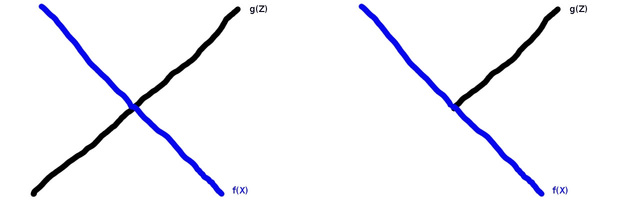
\includegraphics[width=.65\textwidth]{crossingKernel}
    \end{figure}
  \end{block}
\end{frame}

\begin{frame}{Inferring perturbation time II}
\begin{itemize}
\item Hyperparameters are estimated by assuming the two functions are independent, that is they do not cross.
\item Model used "to identify at which time point a gene becomes differentially expressed in time course gene expression data under two various conditions.
\item Both GPy and R implementations are available
\end{itemize}

\begin{block}{Key assumptions}
\begin{itemize}
\item All data points have been labelled as to which function ($f/g$) they belong to.
\item The ordering of time points is assumed known and fixed.
\end{itemize}
\end{block}
\end{frame}



\begin{frame}{Branching Gaussian processes}
\begin{itemize}
\item Extend the kernel to multiple branching points assuming a tree structure. 
\item Infer the function labels.
\item Perform efficient inference (iterative MAP, Variational, Gibbs).
\item Efficient implementation using Google Tensorflow.
\item Time is not given but has be inferred - known as pseudotime inference in single cell literature.
\end{itemize}
\end{frame}


\begin{frame}{Two stage approach}
\begin{itemize}
\item Infer pseudotime [see next slide].
	\begin{itemize}
    	\item Use capture time if available.
\end{itemize}
\item Initialisation: Use overlapping mixture of GPs to infer K trajectories. No branching.
\item Create branching model using OMGP to initialise allocation probabilities $\Phi$ and kernel hyperparameters $\theta$.
	
\item Use Bayesian optimisation (GPyOpt) to learn $\theta$ and branching locations $B$.
	\begin{itemize}
   	\item Currently $\Phi$ fixed but could be optimised locally in each BO step evaluation.
   	\item Still beneficial to use VB code rather than Jings model since we integrate out (approximately using VB bound) uncertainty in allocations.
   	\end{itemize}
\end{itemize}
\end{frame}

\begin{frame}{Pseudotime}
\begin{itemize}
\item Use capture times as informative prior for pseudotime.
	\begin{itemize}
    	\item GPLVM with prior on each point $N(\tau_i | x_i, \sigma^2)$.
	\end{itemize}
\item No capture time.
	\begin{itemize}
    	\item Topslam (GPLVM+)
    	\item Monocle (ICA+mpt)
    	\item Waterfall (PCA+mpt)
    	\item Wanderlust (t-SNE+k-nn).
	\end{itemize}
\item Branching models
	\begin{itemize}
    	\item Diffusion pseudotime.
    	\item Slicer (LLE+entropy criterion).
	\end{itemize}
\end{itemize}
\end{frame}    
    
    

\begin{frame}
\frametitle{Tree prior}
\begin{columns}
\begin{column}{0.7\textwidth} 
    \begin{center}
    Notional prior
     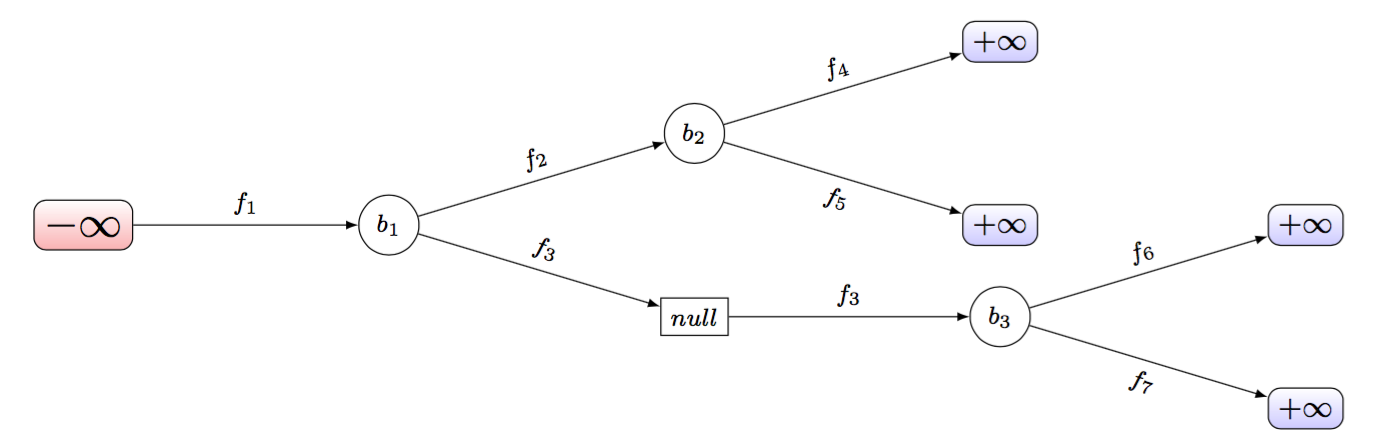
\includegraphics[width=1\textwidth]{branchingGPtreeSmallFL}      
     \end{center}
\end{column}

\begin{column}{0.55\textwidth} 
    \begin{center}
    Sample from the model
     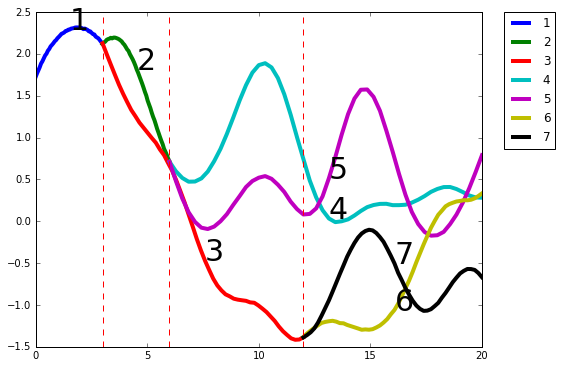
\includegraphics[width=1\textwidth]{multibrachKernelSample}      
     \end{center}
\end{column}
\end{columns}
\end{frame}    

\begin{frame}{Learning pseudotime via Topslam (Max Zwiessele)}
\begin{block}{Density in Bayesian GPLVM}
Probabilistic dimensionality reduction technique allows for estimating the density of the landscape, depicted in gray shading of the background of the two dimensional image of the landscape.  Light areas are preferred by the algorithm, whereas dark areas increase the between cells distance in the landscape.
\end{block}

\begin{block}{Minimum spanning tree}
The extraction of time is done by shortest paths along the extracted graph, depicted in the blue shading of edges, starting from the red circled starting cell.
\end{block}
\end{frame}   

\begin{frame}{Learning pseudotime via Topslam (Max Zwiessele)}
\begin{block}{Key assumptions}
\small
\begin{itemize}
\item Bayesian Gaussian process latent variable model to reduce dimensionality. 
\item Minimum spanning tree to infer pseudotime: temporal order from snapshot view of gene expression.
\end{itemize}
\end{block}

 \begin{center}
 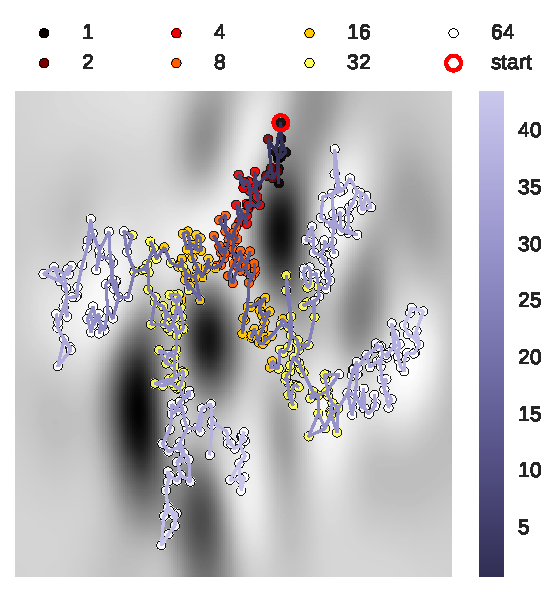
\includegraphics[width=.45\textwidth]{BGPLVMknn50010.pdf}      
 \end{center}
\end{frame}    


\begin{frame}{Step 2: Initialisation in latent space: Overlapping mixture of GPs}
 \begin{center}
 Working on the pseudotime and principal GPLVM direction.
 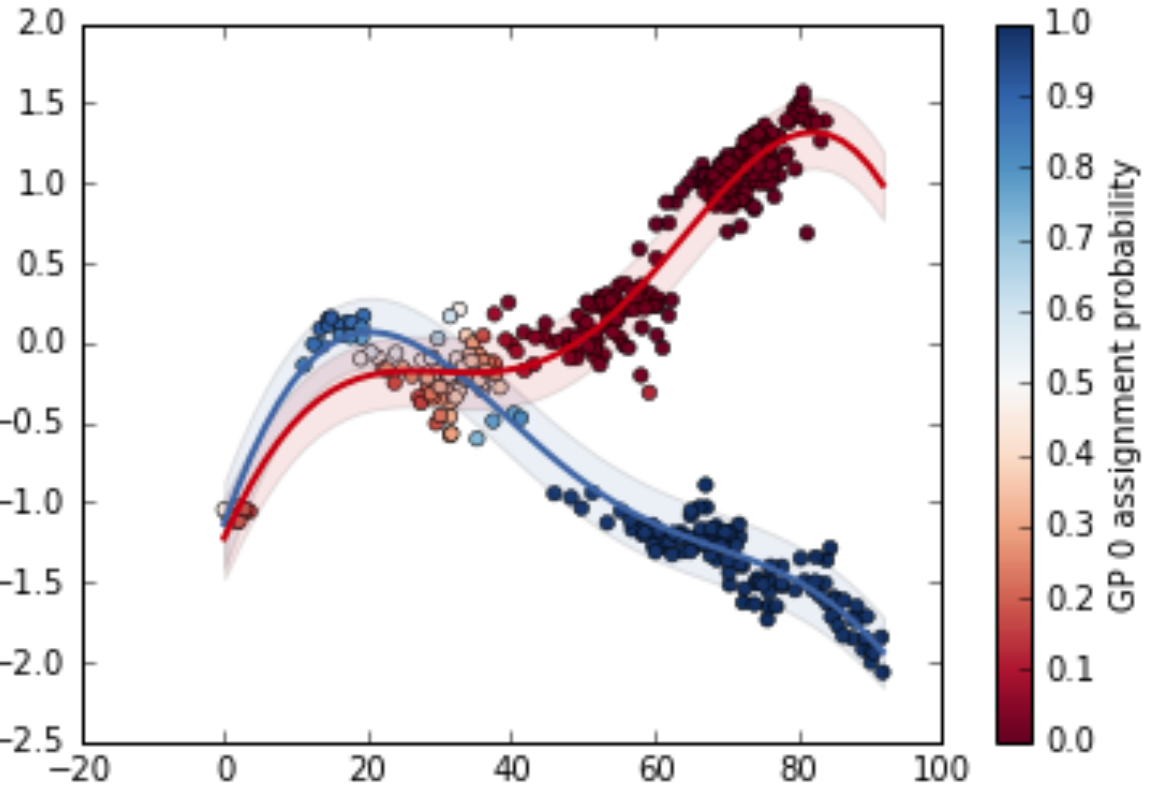
\includegraphics[width=.75\textwidth]{OMGP}      
 \end{center}
\end{frame}    


\begin{frame}{Step 3: Learning the branching structure}
 \begin{center}
 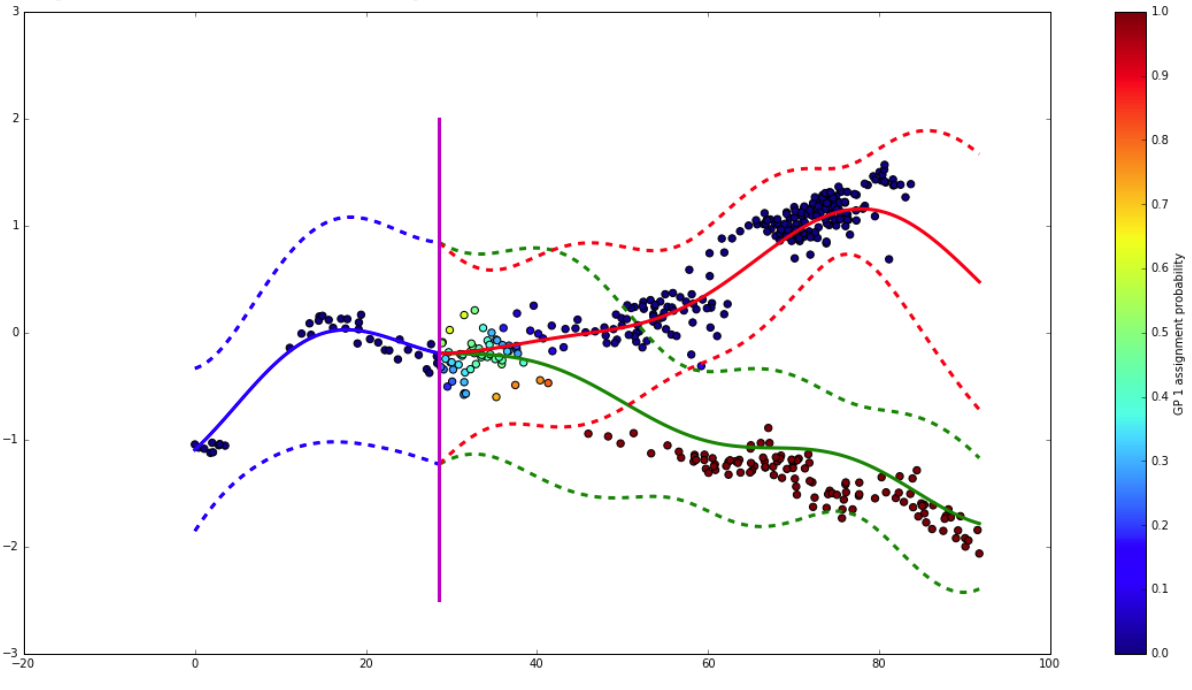
\includegraphics[width=.75\textwidth]{branchingJoint}      
 \end{center}
\end{frame}    

\begin{frame}{Working on the raw gene expression with capture time, gene Id2}
 \begin{center}
 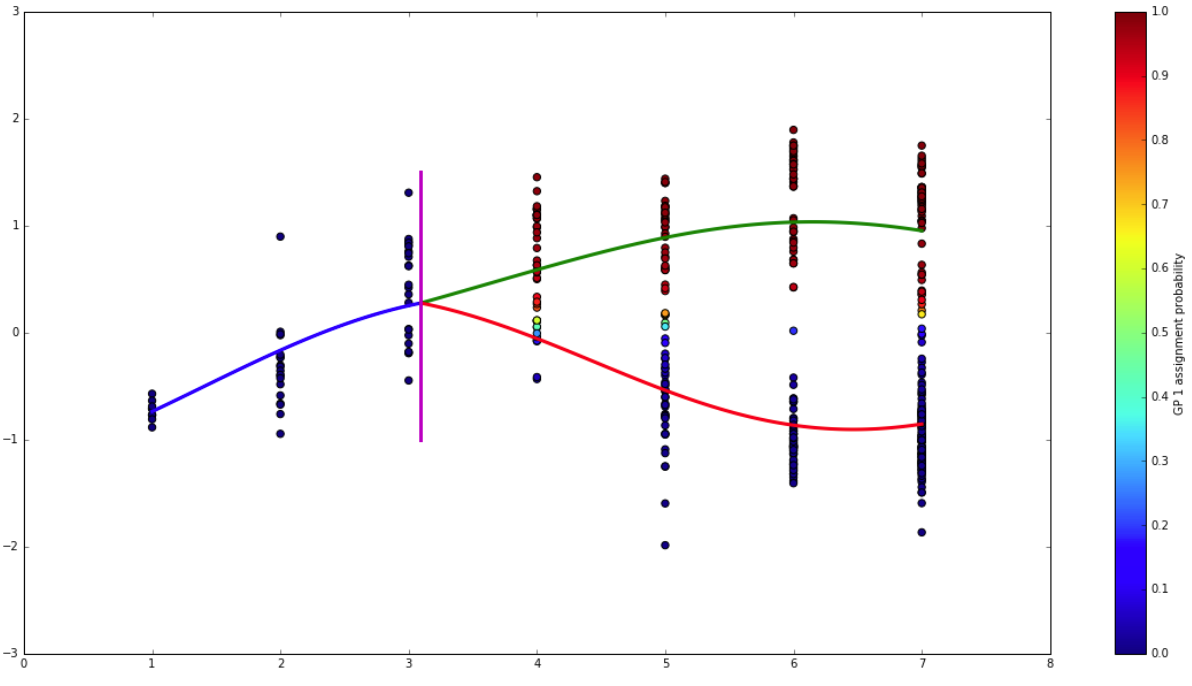
\includegraphics[width=.75\textwidth]{captureTimes}      
 \end{center}
\end{frame}    


\begin{frame}{Raw gene expression: True cell type}
 \begin{center}
 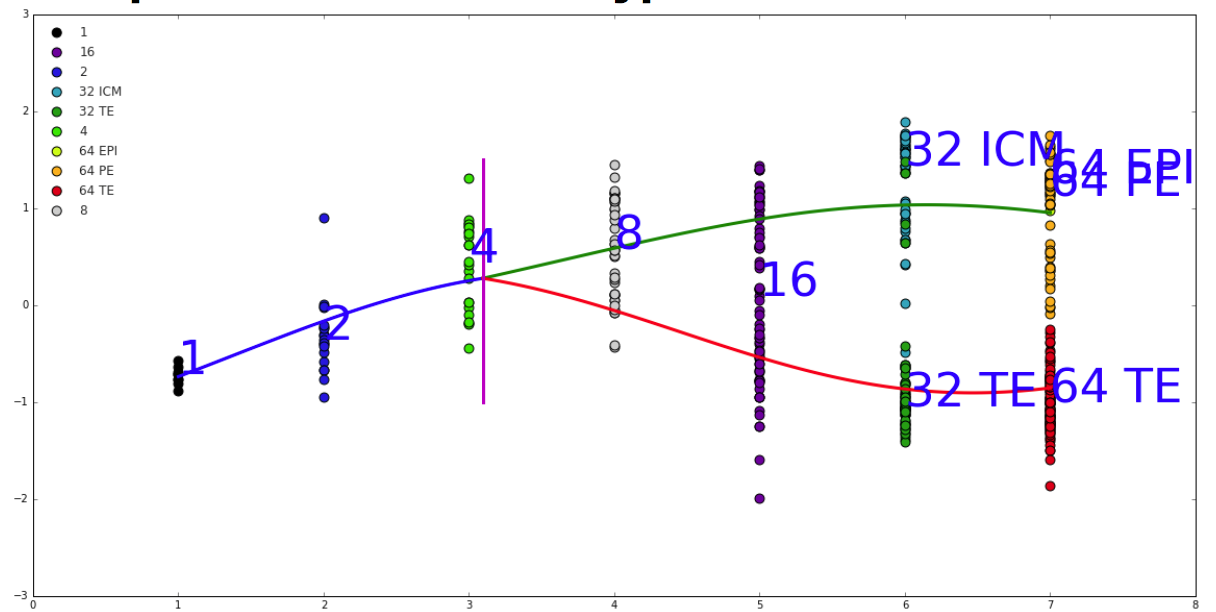
\includegraphics[width=.75\textwidth]{captureTimesGroundTruth}      
 \end{center}
\end{frame}    

   
\begin{frame}{Summary}
\begin{itemize}
\item Infer peudotime across a branching process which allows an unsynchronised or partly synchronised cell population to be placed on a developmental continuum.
\item Easy to extend to multiple branching points: harder optimization problem using same objective function on higher dimensions.
\item Leverage existing approaches (Sparse GP) to improve performance, e.g. Drop-seq=50k cells.
\end{itemize}
\end{frame}   

\begin{frame}{Extensions}
\begin{itemize}
\item Compare to Diffusion pseudotime, Waterfall and Slicer and other approaches.
\item Pseudotime inference; jointly identify labels and time order. 
\item Constrain derivatives to be the same at crossing points so transitions are smooth at branching points.
\item Different kernels in tree structure via model selection; e.g. periodic vs non-periodic kernels.
\item Stochastic process prior on trees. Place non-parametric prior on tree structure and perform inference on tree structure as well as branching GP.
\end{itemize}
\end{frame}    


\end{document}
